\section{State of The Frontend} \label{sec:StateFrontend}

In this section we describe frontend of the WeekPlanner app. This knowledge is based on the code in release version 2018S3R1. 
The frontend code is written in C\#, in the framework Xamarin. The frontend is designed using the \gls{Mvvm} design pattern\ref{fig:MVVM}, where the logic is separated from the user interface. 
From testing the WeekPlaner application it seems to be running somewhat stably,  but the app is lacking in the area of usability. The icons have unclear, and some times multiple, meanings. The user interface is not that aesthetically pleasing, and confusing at times. Some features and customization are also lacking, when using the app interacting with it often feels clunky.
Also a major issue, is that the application only works on the android platform, and many of the current users use Ipads.

\begin{figure}[ht]
    \begin{small}
        \begin{center}
            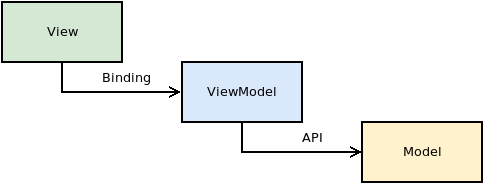
\includegraphics[width=0.75\textwidth]{figures/MVVM_diagram}
        \end{center}
        \caption{Layers in the MVVM pattern}
        \label{fig:MVVM}
    \end{small}
\end{figure}

The View layer contains the user interface, it handles the visual layout. In the \gls{Mvvm} pattern the view layer should only contain logic related to the user interface, and then call functions from the ViewModel when functionality is needed. The ViewModel then contains all necessary functions for communicating between the View layer and the Model layer. When a user for example pushes a button, the button will be connected to a function in the ViewModel through what is called databinding. 
The model contains the data and its representation, and is separated from the ViewModel. 
In the \gls{giraf} “WeekPlanner” project, there is a folder called Views, which contains all Views. Views are also referred to as a page. There is for example a View called LoginPage, which has a Corresponding ViewModel called LoginViewModel. This means when a user has entered a password and username on the login page, the user will pushes a login button. The button is bound to a LoginCommand, which is defined in the LoginViewModel. The function is then called and receives the arguments for the login through the databindings from the View. The ViewModel validates the format of the password and username, and then validates the information through an api that connects with the backend of the system. 
\\
In the following, the folders in the weekplanner will be briefly described.
\\
\textbf{Views:}\\
The Views folder contains all the Views/ pages of the project. This is the user interface part of the system. A lot of the Views are not used for anything. 
\\
\textbf{ViewModels:}\\
The ViewModels folder contains the logic that corresponds to the Views. These will be directly connected. A lot of the Views that correspond with the ViewModels are not used, and therefore the ViewModels are not used.
\\
\textbf{ApplicationObjects:}\\
Contains the setup of an instance of the application. The class “AppContainer” seems to be obsolete. 
\\
\textbf{Behaviors: }\\
Defined behavior for bindings, the bindings utilize the command pattern. 
\\
\textbf{Controls:}\\
Contains a single list view, to be used as a template for a day in the week planner. 
\\
\textbf{Converters:}\\ 
A series of classes used to format data. 
\\
\textbf{Helpers: }\\
A series of helper classes, used in other classes. 
\\
\textbf{Models:}\\
Contains \gls{Dto} for the settings of the app.
\\
\textbf{Services:}\\
Contains some services to e.g.  login, this service can then be used in multiple ViewModels as needed.
\\
\textbf{Themes:}\\
Contains different color themes for the navigation bar.
\\
\textbf{Validation:}\\
Her lies the validation logic for the format of usernames and passwords, if needed new validation rules can be added through constructor injection.